%%%%%%%%%%%%%%%%%%%%%%%%%%%%%%%%%%%%%%%%%
% Stylish Article
% LaTeX Template
% Version 2.1 (1/10/15)
%
% This template has been downloaded from:
% http://www.LaTeXTemplates.com
%
% Original author:
% Mathias Legrand (legrand.mathias@gmail.com) 
% With extensive modifications by:
% Vel (vel@latextemplates.com)
%
% License:
% CC BY-NC-SA 3.0 (http://creativecommons.org/licenses/by-nc-sa/3.0/)
%
%%%%%%%%%%%%%%%%%%%%%%%%%%%%%%%%%%%%%%%%%

%----------------------------------------------------------------------------------------
%	PACKAGES AND OTHER DOCUMENT CONFIGURATIONS
%----------------------------------------------------------------------------------------

\documentclass[fleqn,10pt]{SelfArx} % Document font size and equations flushed left

\usepackage[english]{babel} % Specify a different language here - english by default
\usepackage{lipsum} % Required to insert dummy text. To be removed otherwise
\setlength{\columnsep}{0.55cm} % Distance between the two columns of text
\setlength{\fboxrule}{0.75pt} % Width of the border around the abstract
\definecolor{color1}{RGB}{0,0,90} % Color of the article title and sections
\definecolor{color2}{RGB}{0,20,20} % Color of the boxes behind the abstract and headings
\usepackage{hyperref} % Required for hyperlinks
\hypersetup{hidelinks,colorlinks,breaklinks=true,urlcolor=color2,citecolor=color1,linkcolor=color1,bookmarksopen=false,pdftitle={Title},pdfauthor={Author}}
\usepackage{algorithm}
\usepackage{algorithmic}
\usepackage{multirow}
\usepackage{amsmath}
\usepackage{amssymb}
\def\Plus{\texttt{+}}	
\def\Minus{\texttt{-}} 
\usepackage{amsfonts}
\usepackage{alltt}
\usepackage{url}
\usepackage{relsize}
\usepackage{float}

%----------------------------------------------------------------------------------------
%	ARTICLE INFORMATION
%----------------------------------------------------------------------------------------

\JournalInfo{Computer Science\\School of Informatics, Computing, and Engineering\\Indiana University, Bloomington, IN, USA} % Journal information
\Archive{Datamining B565 Fall 2017}  % Additional notes (e.g. copyright, DOI, review/research article)

\PaperTitle{Kaggle Competitions:\\ \ Author Identification\\ \ Statoil/C-CORE Iceberg Classifier Challenge} % Article title

\Authors{Jinju Jiang, Khushboo Sah, Shreejith Panicker} % Authors
\affiliation{\textsuperscript{1}\textit{Data Science, School of Informatics, Computing, and Engineering, Indiana University, Bloomington, IN, USA}} % Author affiliation

\Keywords{Datamining --- Kaggle --- Neural Network --- CNN --- Naive Bayes --- Image Processing --- TensorFlow} % Keywords - if you don't want any simply remove all the text between the curly brackets
\newcommand{\keywordname}{Keywords} % Defines the keywords heading name
\usepackage{abstract}

%----------------------------------------------------------------------------------------
%	Executive Summary
%----------------------------------------------------------------------------------------

\Abstract{\textbf{Executive Summary}  \\
We have worked on solving two problems from the Kaggle competition using Datamining algorithms and processes.\\
\textbf{Author Identification: }In this problem, we have been given a training data set of excerpts from the Authors Edgar Allan Poe, Mary Shelley, and HP Lovecraft. We have been tasked to classify a test data set of excerpts as belonging to which Author.\\
For this problem we have identified three solutions with varying degrees of success.
\begin{enumerate}
	\item \textbf{Naive Bayes Classifier:}\\
	The Naive Bayes classifier is a simple classifier which works on the premise of conditional independence attributed to Bayes Law. On this premise it classifies each word as belonging to a particular author solely on probability.
	We removed unwanted data in the form of stop words, punctuation and non-Ascii values.\\
	\textit{Results:} We have achieved a consistent accuracy between 84\% to 86\%.
	\item \textbf{Viterbi Algorithm:}\\
	This was inspired by the Naive Bayes classifier, we though we could go a step further with respect to accuracy.
	The Viterbi Algorithm, given a Hidden Markov Model and a set of observations attempts to get the sequence of observations with the Maximum Aposterior Probability.\\
	We implemented it but to our chagrin it didn't perform even remotely as well as the Naive Bayes classifier, we believe it is due to the visualization of the problem.\\
	\textit{Results:} We have achieved a consistent accuracy between 67\% to 70\%.
	\item \textbf{Neural Network:}\\
	We attempted a neural network, as we have known that they are quite robust and accurate when we have sufficient amounts of training data.\\ We implemented the neural network using Keras and Tensorflow packages.\\
	We analysed accuracy with a variety of number of layers, iterations, optimizers and activation functions\\
	\textit{Results:} We have achieved a consistent accuracy between 89\% to 93\%.
\end{enumerate}
\textbf{Statoil/C-CORE Iceberg Classifier Challenge:} In this problem we have been given the data of ice-bergs and ship images, and their incidence angles. Post training of data, we have to classify a new set of data as being icebergs or ships.\\
Having had success with neural networks in the previous problem, we decided to go for this method from the get go.
\begin{enumerate}
	\item \textbf{Convolution Neural Network:} We implemented a CNN here as it is optimal for visual imagery, and we have a huge amount of training data, all of which are very optimal for the implementation of a neural network.\\
	\textit{Results:} We have achieved a consistent accuracy between 84\% to 87\%.
\end{enumerate}
}


\begin{document}

\renewcommand{\abstractname}{}  
\renewcommand{\absnamepos}{} 

\flushbottom % Makes all text pages the same height
\maketitle % Print the title and abstract box
\tableofcontents % Print the contents section
\thispagestyle{empty} % Removes page numbering from the first page

%----------------------------------------------------------------------------------------
%	ARTICLE CONTENTS
%----------------------------------------------------------------------------------------

\section{Introduction}
We are working on a solution for two problems from the Kaggle competition.
\begin{enumerate}
	\item Spooky Author Identification
	\item Statoil/C-CORE Iceberg Classifier Challenge
\end{enumerate}
These problems can be posed as supervised machine learning problems ad we have been given a train and test data-set.\\
To give a brief about \textit{supervised machine learning}\footnote{supervised machine learning is the process of training a machine to identify patterns and possible solutions to a problem based on prior knowledge, i.e. we train the machine on a set of clean and classified data-label set, which is used by the machine to later classify unlabelled data.}.
Datamining is the superset of machine learning algorithmns, it is a vast field which encompasses the process of gathering data, cleaning it, structuring it and labelling it. Machine learning is used only in the final steps. The main function of datamining, as the name would suggest is to mine the data to gather more useable and useful information.\\
E.g.:- By mining the shopping data of a user, we can gather patterns and intents from it. A user maybe browsing for a camera or camera accesories, by mining this users data we can predict that the user intends to purchase a camera. We could then match the user on the basis of his search criteria to the best fit camera.\\
This seems simple, but the process involved is huge.
\begin{enumerate}
	\item Identify relevant searches of user
	\item clean the searches to gather key-words and intents
	\item identify key-words and intents
	\item match the same to relevant objects	
\end{enumerate}
This is just a short description of Dataming and a very simplified one at that.\\We can use the process and algorithms encompassed in datamining to solve the kaggle projects.
\begin{enumerate}
	\item Clean the training data
	\item Train the algorithm using the data
	\item Generate the outcome for the test-data
\end{enumerate}
We have used datamining for all the above steps while working on the kaggle projects.\\
\subsection{Spooky Author Identification}
We have to identify an author from whose works an unlabeled excerpt has been taken.
We have been given a training file containing the labeled excerpts for thw following authors.\\
Edgar Allen Poe, Mary Shelly and HP Lovecraft.\\
We have to identify the pattern of writing (prose, grammar, etc.) of each author, inorder to attempt labeling the test-data.\\
The train data is in the following format.\\
id, text, author\\
The test data is in the following format.\\
id, text\\
The text portion of the data is an excerpt from the works of one of the Authors, e.g.:
\begin{quote}
	Once upon a midnight dreary, while I pondered, weak and weary, Over many a quaint and curious volume of forgotten lore—While I nodded, nearly napping, suddenly there came a tapping, As of some one gently rapping, rapping at my chamber door.“’Tis some visitor,” I muttered, “tapping at my chamber door— Only this and nothing more.”
\end{quote}from Edgar Allen Poe's, \textit{The Raven}. \\
The text has a variety of issues at first glance itself.\\
We have had to clean the data to get it to run in our implemented solutions.
\begin{itemize}[noitemsep]
	\item Common Words : There are a lot common words associated with each author, we filtered them out.
	\item Punctuation : Punctuation tends to convert the same word into a variety of forms (Eg: cat, cat's), we removed them so that we can get larger probabilities for the words.
	\item Presence of non-ASCII values : There were certain non-ASCII values, which interfere with the probability calculations, we have removed them.
\end{itemize}
\subsection{Statoi/C-CORE Iceberg Classifier Challenge}
The Iceberg classifier challenge is a visual data processing challenge. In this challenge, we have to identify based on certain visual data inputs whether an image contains and iceberg or not.\\
We have been provided train data in the json format, containing the following fields.\\
id - image id\\
band\_1,band\_2 - Flattened image data of 75X75 pixels, i.e. 5625 elements, which were signals, corresponding to how the images were transmitted and recieved\footnote{Band 1 and Band 2 are signals characterized by radar backscatter produced from different polarizations at a particular incidence angle. The polarizations correspond to HH (transmit/receive horizontally) and HV (transmit horizontally and receive vertically). More background on the satellite imagery can be found here.}.\\
inc\_angle - The incidence angel at which the image was taken.\\
is\_iceberg - Classifier column, for the training data.\\
The test data has all the same fields except the last one which is to be evaluated and provided by use via our processing.\\
We haven't had to clean the data much, except for the inc\_angle field containing a few NULL values, which actually work to our advantage as they are all icebergs.\\
We need to process all this visual data to discern patterns to identify icebergs as accurately as possible.
\section{Datamining}
Data mining is the computing process of discovering patterns in large data sets involving methods at the intersection of machine learning, statistics, and database systems.It is an essential process where intelligent methods are applied to extract data patterns.It is an interdisciplinary subfield of computer science.The overall goal of the data mining process is to extract information from a data set and transform it into an understandable structure for further use. Aside from the raw analysis step, it involves database and data management aspects, data pre-processing, model and inference considerations, interestingness metrics, complexity considerations, post-processing of discovered structures, visualization, and online updating.Data mining is the analysis step of the "knowledge discovery in databases" process.\

There are various steps that are involved in mining data as shown in the picture.
\begin{figure}[ht]\centering
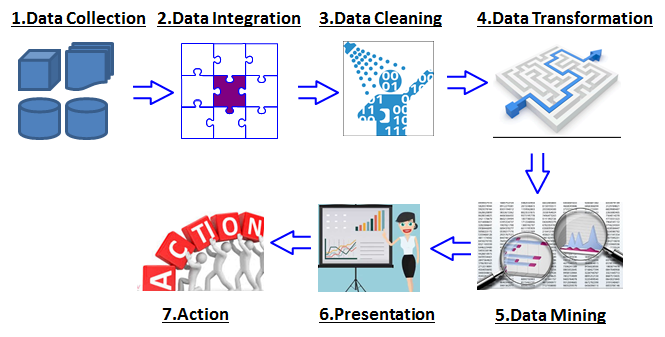
\includegraphics[width=\linewidth]{Dataminingsteps}
\caption{Data mining steps}
\label{fig:Dataminingsteps}
\end{figure}
\begin{enumerate}
\item Data Collection: First of all the data are collected from all the different sources.
\item Data Integration: involves combining data residing in different sources and providing users with a unified view of them.
\item Data Cleaning: The data we have collected are not clean and may contain errors, missing values, noisy or inconsistent data. So we need to apply different techniques to get rid of such anomalies.
\item Data Transformation: The data even after cleaning are not ready for mining as we need to transform them into forms appropriate for mining. The techniques used to accomplish this are smoothing, aggregation, normalization etc.
\item Data Mining: Now we are ready to apply data mining techniques on the data to discover the interesting patterns. Techniques like clustering and association analysis are among the many different techniques used for data mining. 
\item Pattern Evaluation and Knowledge Presentation: This step involves visualization, transformation, removing redundant patterns etc from the patterns we generated.
\item Decisions / Use of Discovered Knowledge: This step helps user to make use of the knowledge acquired to take better decisions.
\end{enumerate}

Data clustering and classification are 2 major method used in data mining.Cluster analysis or clustering is the task of grouping a set of objects in such a way that objects in the same group (called a cluster) are more similar (in some sense or another) to each other than to those in other groups (clusters).Data classification is the process of organizing data into categories for its most effective and efficient use. Here it is the difference between clustering and classification.
\begin{figure}[ht]\centering
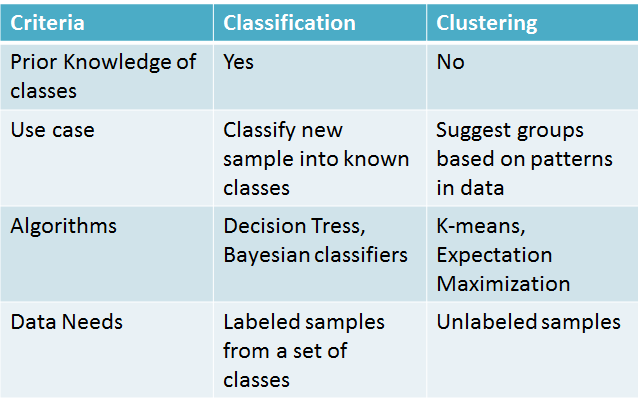
\includegraphics[width=\linewidth]{classification}
\caption{Clustering vs Classification}
\label{fig:classification}
\end{figure}

Loss functions define how to penalize incorrect predictions. The optimization problems associated with various linear classifiers are defined as minimizing the loss on training points (sometime along with a regularization term).


\subsection{Data Preprossing}

Data preprocessing is a data mining technique that involves transforming raw data into an understandable format. Real-world data is often incomplete, inconsistent, and/or lacking in certain behaviors or trends, and is likely to contain many errors. Data preprocessing is a proven method of resolving such issues. Data preprocessing prepares raw data for further processing.It involves several steps as the following:
\begin{itemize}[noitemsep]
\item Data cleaning: fill in missing values, smooth noisy data, identify or remove outliers, and resolve inconsistencies.
\item Data integration: using multiple databases, data cubes, or files.
\item Data transformation: normalization and aggregation.
\item Data reduction: reducing the volume but producing the same or similar analytical results.
\item Data discretization: part of data reduction, replacing numerical attributes with nominal ones.
\end{itemize}

Data preprocessing is the most time and cost consuming task. It normally take about 80-90 percent of the whole cost and time.

\subsection{Mining, Interpretation, and Action}
There are a lot of data mining algorithms, the top 10 algorithsms identified are C4.5, k-Means, SVM, Apriori, EM, PageRank, AdaBoost, kNN, Naive Bayes, and CART. These top 10 algorithms are among the most influential data mining algorithms in the research community.
\begin{enumerate}
\item \textbf{C4.5:}\\C4.5 is an algorithm used to generate a decision tree developed by Ross Quinlan.[1] C4.5 is an extension of Quinlan's earlier ID3 algorithm. The decision trees generated by C4.5 can be used for classification, and for this reason, C4.5 is often referred to as a statistical classifier.C4.5 builds decision trees from a set of training data in the same way as ID3, using the concept of information entropy.
\item \textbf{K-Means:}\\K-means clustering is a method of vector quantization, originally from signal processing, that is popular for cluster analysis in data mining. k-means clustering aims to partition n observations into k clusters in which each observation belongs to the cluster with the nearest mean, serving as a prototype of the cluster.
\item \textbf{SVM:}\\support vector machines (SVMs, also support vector networks) are supervised learning models with associated learning algorithms that analyze data used for classification and regression analysis. Given a set of training examples, each marked as belonging to one or the other of two categories, an SVM training algorithm builds a model that assigns new examples to one category or the other, making it a non-probabilistic binary linear classifier.
\item \textbf{Apriori:}\\The Apriori Algorithm is an influential algorithm for mining frequent itemsets for boolean association rules. Apriori uses a "bottom up" approach, where frequent subsets are extended one item at a time (a step known as candidate generation, and groups of candidates are tested against the data. Apriori is designed to operate on database containing transactions (for example, collections of items bought by customers, or details of a website frequentation).
\item \textbf{EM:}\\An expectation–maximization (EM) algorithm is an iterative method to find maximum likelihood or maximum a posteriori (MAP) estimates of parameters in statistical models, where the model depends on unobserved latent variables. The EM iteration alternates between performing an expectation (E) step, which creates a function for the expectation of the log-likelihood evaluated using the current estimate for the parameters, and a maximization (M) step, which computes parameters maximizing the expected log-likelihood found on the E step. These parameter-estimates are then used to determine the distribution of the latent variables in the next E step.
\item \textbf{PageRank:}\\PageRank is an algorithm used by Google Search to rank websites in their search engine results. PageRank was named after Larry Page, one of the founders of Google. PageRank is a way of measuring the importance of website pages.PageRank produces a static ranking of Web pages in the sense that a PageRank value is computed for each page off-line and it does not depend on search queries. The algorithm
relies on the democratic nature of the Web by using its vast link structure as an indicator of an individual page’s quality.
\item\textbf{AdaBoost:}\\AdaBoost, short for Adaptive Boosting, is a machine learning meta-algorithm formulated by Yoav Freund and Robert Schapire, who won the 2003 Gödel Prize for their work. It can be used in conjunction with many other types of learning algorithms to improve performance. The output of the other learning algorithms ('weak learners') is combined into a weighted sum that represents the final output of the boosted classifier. AdaBoost is adaptive in the sense that subsequent weak learners are tweaked in favor of those instances misclassified by previous classifiers. AdaBoost is sensitive to noisy data and outliers.
\item \textbf{K-NN:}\\The k-nearest neighbors algorithm (k-NN) is a non-parametric method used for classification and regression.[1] In both cases, the input consists of the k closest training examples in the feature space.k-NN is a type of instance-based learning, or lazy learning, where the function is only approximated locally and all computation is deferred until classification. The k-NN algorithm is among the simplest of all machine learning algorithms.
\item \textbf{Naive Bayes classifiers:}\\Naive Bayes classifiers are a family of simple probabilistic classifiers based on applying Bayes' theorem with strong (naive) independence assumptions between the features.Naive Bayes is a simple technique for constructing classifiers: models that assign class labels to problem instances, represented as vectors of feature values, where the class labels are drawn from some finite set. It is not a single algorithm for training such classifiers, but a family of algorithms based on a common principle: all naive Bayes classifiers assume that the value of a particular feature is independent of the value of any other feature, given the class variable.
\item \textbf{CART:}\\The CART (Classification And Regression Trees) algorithm is structured as a sequence of questions, the answers to which determine what the next question, if any should be.  The result of these questions is a tree like structure where the ends are terminal nodes at which point there are no more questions.The CART decision tree is a binary recursive partitioning procedure capable of processing continuous and nominal attributes both as targets and predictors. Data are handled in their raw form; no binning is required or recommended.
\end{enumerate}

Data mining, or knowledge discovery, is the computer-assisted process of digging through and analyzing enormous sets of data and then extracting the meaning of the data. There are a lot tools,methods and algorithms, and there are a lot of steps involved. Data mining will not tell what is the best solution, we need to try and search case by case to find the best one.\

The most challenges for data mining now is increasingly Large Volumes of Data.As new applications become increasingly complex, developers are facing greater pressure to process much larger data sets. Some applications require data scientists to extract and analyze multiple petabytes of data. The quantity of data continues to grow faster than the ability of the network to carry it all.

%------------------------------------------------
%
%  Author Identication
%   
%------------------------------------------------
\section{Spooky Author Idenfication: Full Problem Description}
\textbf{Problem:}Identify an author accurately from a set of three, from whose works the unlabeled test excerpt has been taken.\\
Edgar Allan Poe, Mary Shelley, and HP Lovecraft\\
\textbf{Input \& Output}\\
training input : Cleaned training data, without punctuation, stop words and non-ascii characters.\\
training output : Probability or weight and bias distribution required to identify the unlabeled data.\\
test input : Unlabeled cleaned data from test file.\\
test output : Probability of excerpt belonging to which author.\\
\textbf{Training \& Testing Methods}\\
\textbf{Naive Bayes Classifier:} Create a probability distribution of the words given author and the words themselves. Identifies the individual word-author association in the test data to give a label.\\
\textbf{Viterbi Algorithm:} Creates emission, transition and initial probabilities of the authors and words based on assumption that authors are a HMM. Identifies the sequence of authors which is maximum for a given test-excerpt and finally assigns the author who is maximized.\\
\textbf{Neural Network:} Uses the training inputs to correctly assign weights and bias to each neuron in the network. Identifies the author for the test-data based on the trained weights and bias.

\subsection{Data Analysis}
\begin{itemize}[noitemsep]
\item Describe the data in full detail--from its raw form to the transformation
\item Provide summary statistics and relationships

\begin{figure}[H]\centering
	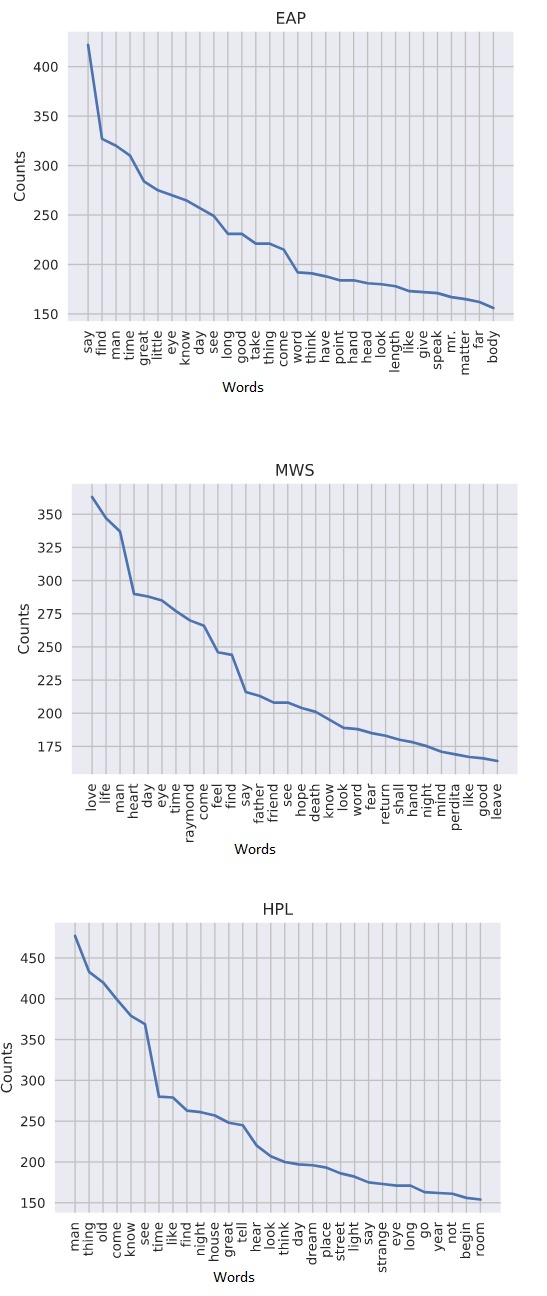
\includegraphics[width=\linewidth]{merge_from_ofoct.jpg}
	\caption{This graph shows few sample word frequency for each author in training file}
	\label{fig:Word frequency Author}
\end{figure}

\begin{figure}[H]\centering
	\includegraphics[width=\linewidth]{DistAuthor.jpeg}
	\caption{This graph shows count of each author in training file is approximately equal}
	\label{fig: Author count in training file}
\end{figure}
We can see from the above analysis that there is no bias introduced in the data by one Author being less represented than the other, all are almost equal.\\
\end{itemize}



\subsection{Methods}
We have chosen the following algorithms for implementation in the order of implementation
\begin{enumerate}
	\item Naive Bayes Classifier
	\item Viterbi Classification
	\item Neural Network
\end{enumerate}
\subsubsection{Naive Bayes Classifier}
We have chosen the Naive Bayes Classifier for the initial implementation because
\begin{itemize}[noitemsep]
	\item It is simple to implement.
	\item Works well with natural language processing.
	\item It is able to handle missing data quite well.
	\item Due to it's simple calculations, it is inherently quick.
	\item It is able to reliably handle large inputs.
\end{itemize}
We had made an implementation using Naive Bayes to classify tweets with respect to location and this problem of mapping authors to a given sentence was very similar.
We have had exposure ww=orking on Naive Bayes classifier in our Artificial Intelligence course. We know Naive Bayes is based on Bayes Law of conditional independence. Basically, Naive Bayes assumes that every word which we encounter is independent in it's occurrence given the author.\\
In our implementation we calculate the prior and the likelihood of the word given the author and store it. These probabilities are use to calculate the posterior probability of the word being associated with an author while testing.\\
\begin{equation}
P(Author/Word) =\frac{P(Word/Author)*P(Author)}{P(Word)}
\label{eq:refname3}
\end{equation}
\\
We faced the following challenges while working
\begin{itemize}[noitemsep]
	\item Common Words : There are a lot common words associated with each author, we filtered them out.
	\item Punctuation : Punctuation tends to convert the same word into a variety of forms (Eg: cat, cat's), we removed them so that we can get larger probabilities for the words.
	\item Presence of non-ASCII values : There were certain non-ASCII values, which interfere with the probability calculations, we have removed them.
	\item Probability calculations exceed python float range : The calculations became very tiny, we converted them into logarithms to be able to process them.
\end{itemize}
We have used the following software and hardware.\\
\textbf{Software}
\begin{itemize}[noitemsep]
	\item Python 3.5.2
	\item Sublime Text 3
\end{itemize}
\textbf{Hardware}
\begin{itemize}[noitemsep]
	\item Model : Dell Inspiron 7559 Signature Edition
	\item Processor :Intel core-i7
	\item System type : Windows 10 64 bit operting system
	\item RAM : 16 GB
\end{itemize}
\textbf{Train \& Test Visualization}\\
\begin{figure}[H]\centering
	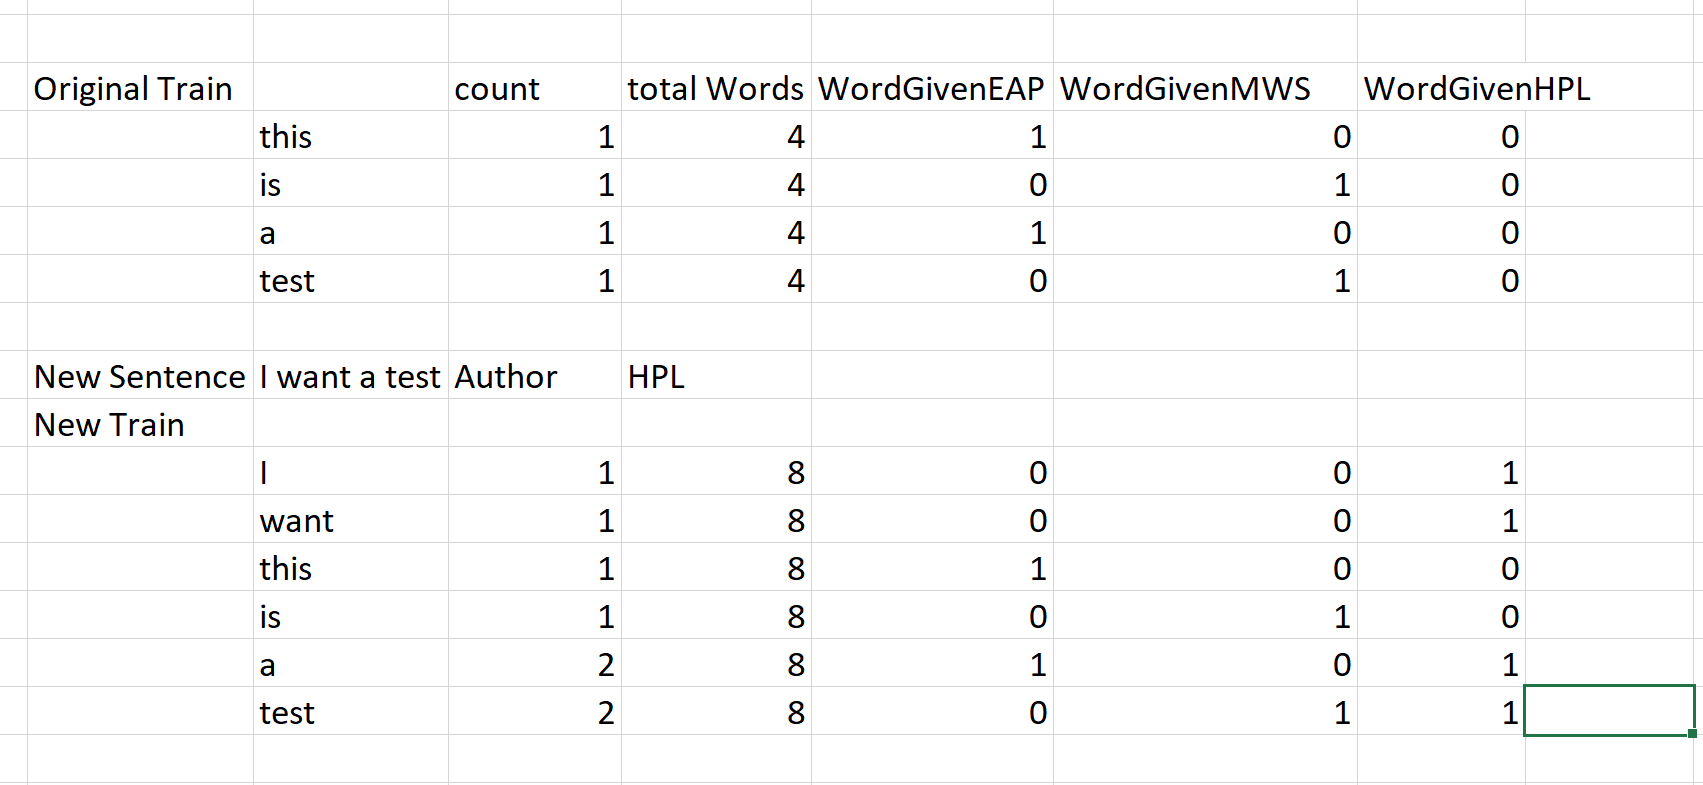
\includegraphics[width=\linewidth]{TrainingNaiveBayes.PNG}
	\caption{Naive Bayes Training}
	\label{fig:Naive Bayes Training}
\end{figure}
\begin{figure}[H]\centering
	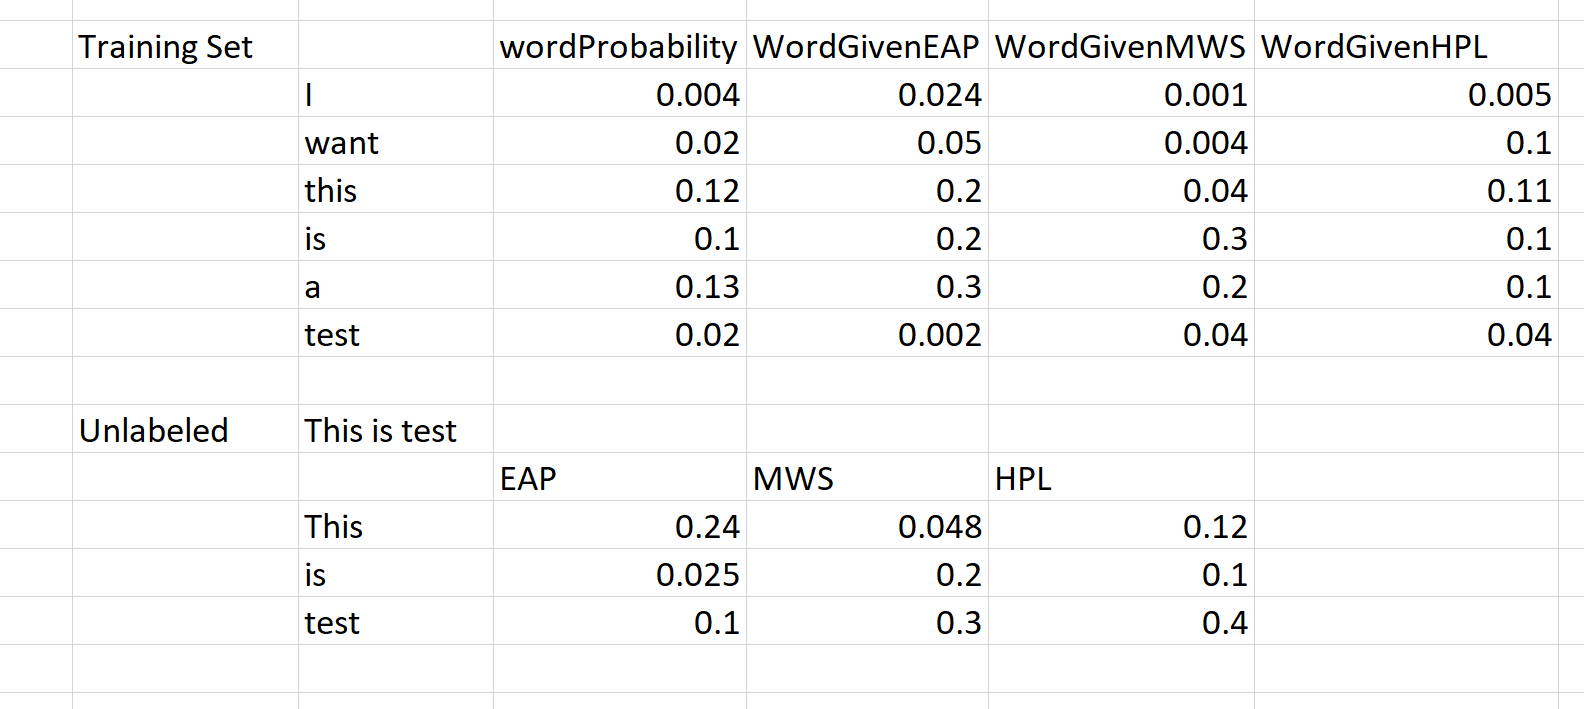
\includegraphics[width=\linewidth]{TestNaiveBayes.PNG}
	\caption{Naive Bayes Test}
	\label{fig:Naive Bayes Test}
\end{figure}
Please note the values in the figures of training and testing are arbitary only to show the working of the implementation.\\
\subsubsection{Viterbi Algorithm}
The Viterbi Algorithm was inspired by the naive bayes classifier. While working on a similar implementation in the Artificial Intelligence course, we saw a similarity between the problem we were working on and the Spooky Author Identification. We discussed this with Prof. Dalkilic and he was enthusiastic for us to give it a try.\\
We choose it for the following reasons
\begin{itemize}[noitemsep]
	\item It builds upon naive bayes.
	\item It identifies the maximum sequence of states, here we can identify the maximized author associated with each sentence.
\end{itemize}
Viterbi algorithm is used inorder to find the Maximum Aposterior Probability, i.e. given a hidden Markov Chain and a set of observations, it calculates the sequence of observations with the maximum probability of occurence.\\
We visualized this a little for our implementation, we said every sentence has a HMM in the form of initial probability, transition probability and emission probability with respect to the Authors and the Words.\\
Using these we evaluated for a given sentence the maximum author sequence which will be generated, the sequence would then be broken down to evaluate which author featured most and that author would be assigned to the given sentence.\\
We faced the following challenges while working
\begin{itemize}[noitemsep]
	\item Punctuation : Punctuation tends to convert the same word into a variety of forms (Eg: cat, cat's), we removed them so that we can get larger probabilities for the words.
	\item Presence of non-ASCII values : There were certain non-ASCII values, which interfere with the probability calculations, we have removed them.
	\item Probability calculations exceed python float range : The calculations became very tiny, we converted them into logarithms to be able to process them.
\end{itemize}
We have used the following software and hardware.\\
\textbf{Software}
\begin{itemize}[noitemsep]
	\item Python 3.5.2
	\item Sublime Text 3
\end{itemize}
\textbf{Hardware}
\begin{itemize}[noitemsep]
	\item Model : Dell Inspiron 7559 Signature Edition
	\item Processor :Intel core-i7
	\item System type : Windows 10 64 bit operting system
	\item RAM : 16 GB
\end{itemize}
\textbf{Train \& Test Visualization}\\
\begin{figure}[H]\centering
	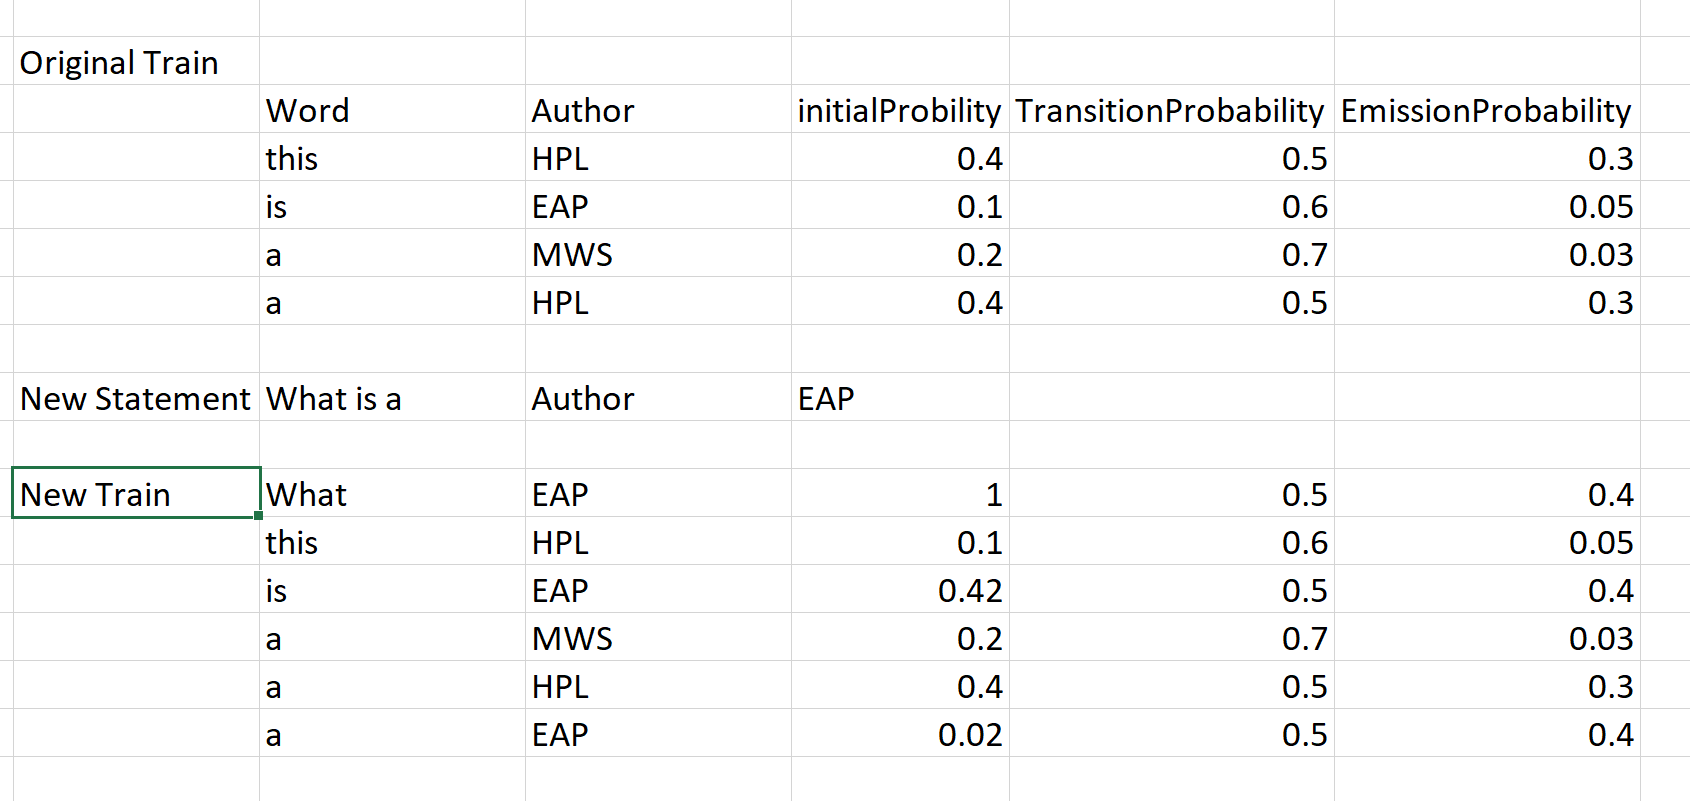
\includegraphics[width=\linewidth]{ViterbiTrain.png}
	\caption{Viterbi Training}
	\label{fig:Viterbi Training}
\end{figure}
\begin{figure}[H]\centering
	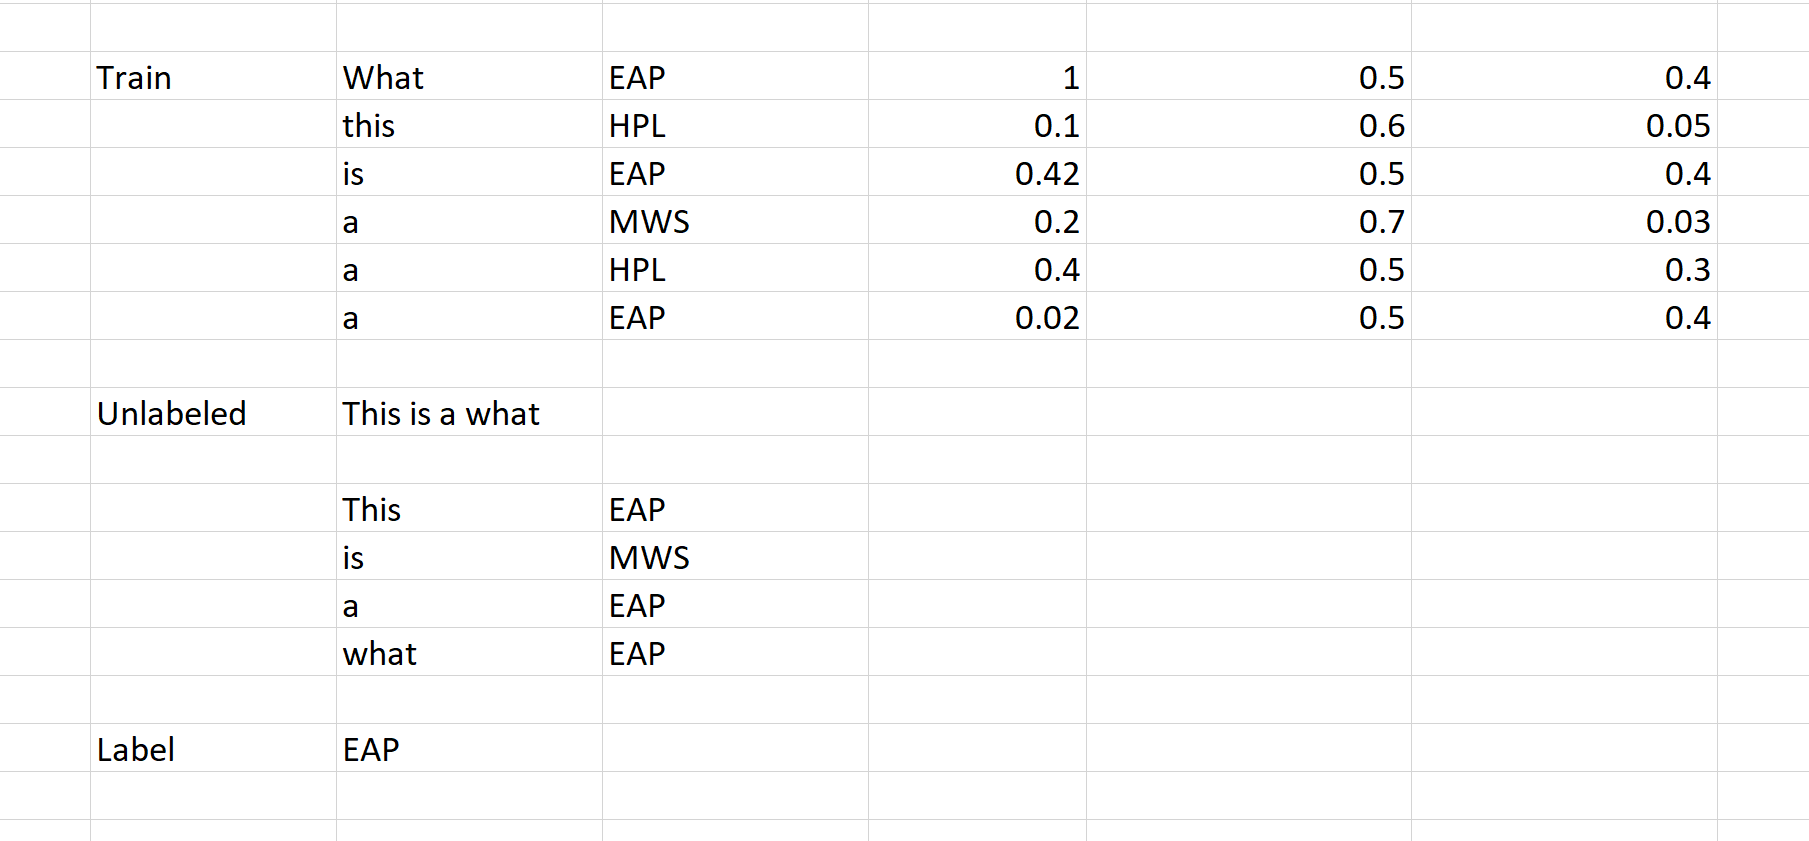
\includegraphics[width=\linewidth]{ViterbiTest.png}
	\caption{Viterbi Test}
	\label{fig:Viterbi Test}
\end{figure}
Please note the values in the figures of training and testing are arbitary only to show the working of the implementation.\\
\subsubsection{Neural Network}
We decided to go for a third implementation for the Spooky Author Classification, because we weren't satisfied with the results we got for our previous implementation.\\
We discussed as to what we should choose to get better results and neural networks was something we all wanted to try. Hence, we went for neural networks.\\
There are some salient advantages as well\\
\begin{itemize}[noitemsep]
	\item High accuracy, especially if enough data is present.
	\item Very fast classification.
	\item It is also one of the most cutting edge when it comes to machine learning.
\end{itemize}
Neural networks work as follows:\\
There are 2 layes which interact with the world (i.e. outside of the network), namely the input layer and the output layer, each of which has n neurons. In our implementation we have chosen one neuron for every fifteen rows of data, and have three neurons for the output layer associated with each of the Authors. Apart from these two layers, the neural network can have an infinite number of hidden layers, for our implementation we have chosen two hidden layers, each with the same number of neurons as in the input layer.\\
We have implemented a simple feed-forward neural network, where every previous layer's neuron is connected to every current layer's neuron and the data is fed-forward till it reaches the output layer.\\
The initial weights and bias in the network is randomized and as the network processes the training data it "learns" and corrects itself, finally reaching a set of weights and bias for each neuron, we use feed-forward to process the data and backward propagation to correct the weights and bias.\\
The final network is then run on the test data. We have implemented this using the keras package for the neural network and tensorflow for performance.\\
We faced the following challenges while implementing it.
\begin{itemize}[noitemsep]
	\item Choosing a proper activation function: We saw that the sigmoid was performing below par and could eke out a bit more accuracy using the softmax
	\item Choosing an optimizer: We played with the available optimizers in keras and finally settled on ADAM
	\item Performance issues: The initial implementation was running a bit too slow, we decided to use tensorflow to improve performance.
\end{itemize}
We have used the following software and hardware.\\
\textbf{Software}
\begin{itemize}[noitemsep]
	\item Python 3.5.2
	\item Sublime Text 3
	\item numpy
	\item pandas
	\item keras
	\item tensorflow
\end{itemize}
\textbf{Hardware}
\begin{itemize}[noitemsep]
	\item Model : Dell Inspiron 7559 Signature Edition
	\item Processor :Intel core-i7
	\item System type : Windows 10 64 bit operting system
	\item RAM : 16 GB
\end{itemize}

%------------------------------------------------

\subsection{Results}
\begin{itemize}[noitemsep]
\item Dispassionately describe your results both quantified and qualified
\item Do you deem this successful
\item What do the results suggest
\item What were challenges
\end{itemize}
Remember, we're interested in the journey, so simply because an approach failed doesn't mean failure if you discuss the failure!

Please see a summary of the results that we have obtained, I will go into the details of each as well.\\
\begin{figure}[H]\centering
	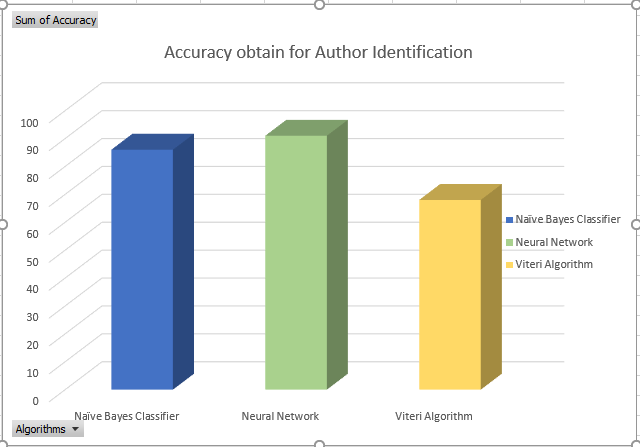
\includegraphics[width=\linewidth]{Accuracy.PNG}
	\caption{Results of the Spooky Author Solutions}
	\label{fig:Results}
\end{figure}
\textbf{Naive Bayes Classifier:}\\
The naive bayes classifier has really delivered, a simple classifier augmented with a little clean-up has given around 87\% accuracy consistently.\\
We believe this was a success. We think this can attributed to the simple fact that Bayes Law works.\\
We did have a ton of challenges, removing the non-ascii characters, punctuation and stop-words, which we believe has improved both performance and accuracy.\\
Statistics for Naive Bayes Classifier\\
Accuracy : 84\% - 86\% \\
Time for training : 20 seconds \\
Time for testing : 10 seconds \\
\\
\textbf{Viterbi Algorithm: }\\
The viterbi algorithm was a disappointment, let alone improving it wasn't even at par with a much simpler classifier like naive bayes. We believe this can be attributed to the issue that Viterbi Algorithm just wasn't suited for this problem.\\
The visualization for the initial, transition and emission probabilities were a bit off mark.\\
We also have another suspision regarding the failure, which is the training data is insufficient w.r.t. Viterbi. We noted that there was an improvement in the accuracy if more of the train data was used for training instead of testing.\\
Statistics for Viterbi Algorithm\\
Accuracy : 67\% - 70\% \\
Time for training : 58 seconds \\
Time for testing : 20 seconds \\
\\
\textbf{Neural Network: }\\
This is also a success story and a much better accuracy then with the other implementations. We believe this is due to the nature of the neural network itself, as it's complexity increases so does it's capacity to learn. We saw this markedly, when we increased the number of epochs (iterations) and the accuracy kept increasing, until leveling at 25 epochs.\\
We would love to further work on this to evaluate if any further significant increase is possible.\\
Statistics for Neural Network\\
Accuracy : 90\% - 93\% \\
Time for training : 120 seconds \\
Time for testing : 20 seconds \\
\\
We tested the data using a 10-Fold cross validation.\\
We randomly created test and train data from the cleaned training data, using 30\% for test and rest for train.\\
\subsection{Summary and Future Work}
The Spooky Author Identification was a fun project to work on. It really helped us visualize the various aspects of Datamining personally.Working with textual data is really refreshing and investigating various algorithms is really a good way to improve knowledge base.\\
To Summarize, the spooky author identification Kaggle project required us to label unlabeled excerpts for three authors, using trained data of properly labeled excerpts.\\
We attempted to solve this using naive bayes classifier, viterbi algorithm and neural networks and were successful in achieving an accuracy of 91\% (neural network).\\
With respect to future work we would like to list the following, time just wasn't enough with the finals week for us to attempt these.
\begin{enumerate}
	\item Attempt Lemmatizing words as part of clean-up.
	\item Implement Naive Bayes Classifier using TF-IDF package instead of counting frequency.
	\item Investigate causes of failure for Viterbi Algorithm.
	\item Attempt NLP and text2Vec for this problem.
\end{enumerate}
\section{Iceberg: Full Problem Description}

Drifting icebergs caused risks to navigation and activities. Companies are using all kinds of methods to sense and monitor in order to detect the threatening icebergs as early as possible. One method is to use Satellite radar to detect it:  It bounces a signal off an object and records the echo, then that data is translated into an image. An object will appear as a bright spot because it reflects more radar energy than its surroundings, but strong echoes can come from anything solid - land, islands, sea ice, as well as icebergs and ships. The energy reflected back to the radar is referred to as backscatter.When the radar detects a object, it can't tell an iceberg from a ship or any other solid object. The object needs to be analyzed for certain characteristics - shape, size and brightness - to find that out.\

What we need to do is to use data with two channels: HH (transmit/receive horizontally) and HV (transmit horizontally and receive vertically) to figure out whether it is a ship or iceberg.The following picture will show what we will to detect the iceberg:
\begin{figure}[ht]\centering
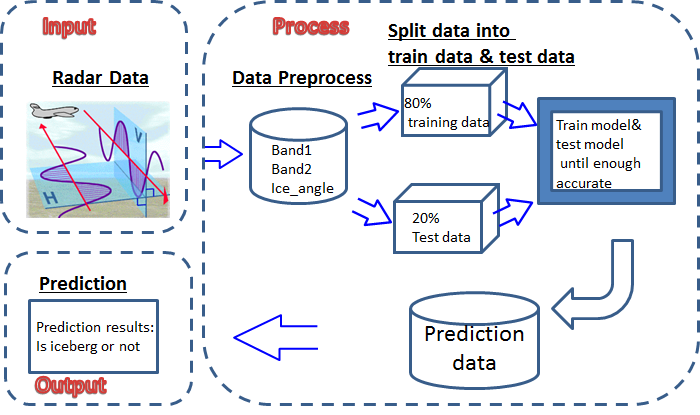
\includegraphics[width=\linewidth]{p2inputoutput}
\caption{Here it is how we will resolve this problem to detect the iceberg.}
\label{fig:p2inputoutput}
\end{figure}


\subsection{Data Analysis}
First let's load data into MS SQL 2016 database:

\begin{figure}[ht]\centering
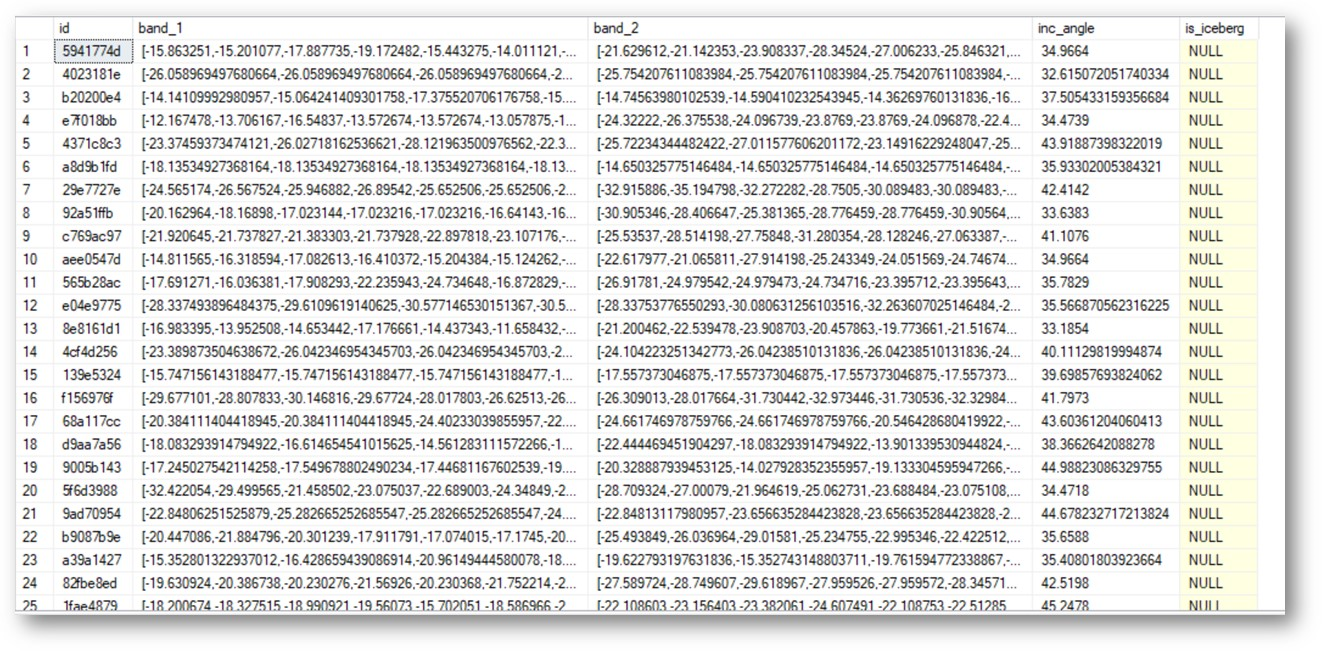
\includegraphics[width=\linewidth]{sql}
\caption{data is loaded into SQL 2016}
\label{fig:sql}
\end{figure}
We got the following training data with 5 variables for train data and 4 variables(no target variable) for testing data:\\
\underline{$id$} - the id of the image\\
\underline{band\_1, band\_2} - the flattened image data. Each band has $75x75$ pixel values in the list, so the list has 5625 elements. Note that these values are not the normal non-negative integers in image files since they have physical meanings - these are float numbers with unit being dB. Band\_1 and Band\_2 are signals characterized by radar backscatter produced from different polarizations at a particular incidence angle. The polarizations correspond to HH (transmit/receive horizontally) and HV (transmit horizontally and receive vertically). More background on the satellite imagery can be found here.\\
\underline{$inc\_angle$}- the incidence angle of which the image was taken. Note that this field has missing data marked as "na", and those images with "na" incidence angles are all in the training data to prevent leakage.\\
\underline{$is\_iceberg$} - the target variable, set to 1 if it is an iceberg, and 0 if it is a ship.\\
\underline{Firstly},let's analysis band\_1 and band\_2 data since they are the critical data here. \\
Here it is the standard deviation, mean and median analysis for band\_1 and band\_2:\\
\begin{figure}[ht]\centering
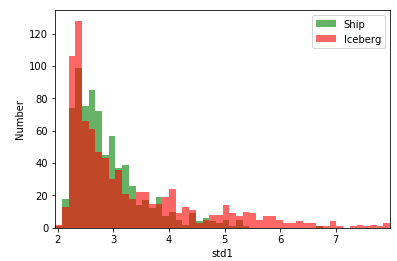
\includegraphics[width=\linewidth]{std1}
\caption{std1 for band\_1: iceberg has wider std than ship}
\label{fig:std1}
\end{figure}
\begin{figure}[ht]\centering
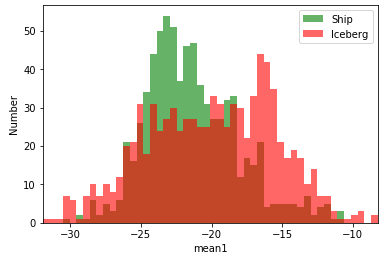
\includegraphics[width=\linewidth]{mean1}
\caption{mean1 for band\_1: iceberg has wider mean than ship}
\label{fig:mean1}
\end{figure}
\begin{figure}[ht]\centering
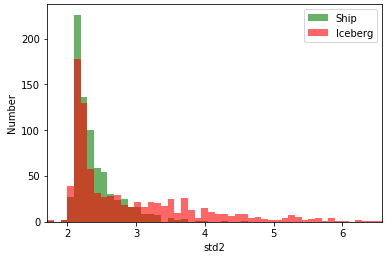
\includegraphics[width=\linewidth]{std2}
\caption{std1 for band\_2: iceberg has wider std than ship,similar as band\_1}
\label{fig:std2}
\end{figure}
\begin{figure}[ht]\centering
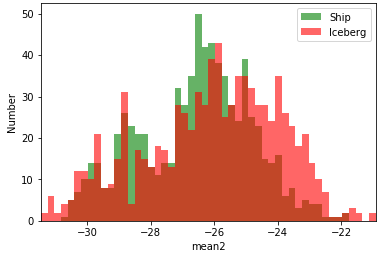
\includegraphics[width=\linewidth]{mean2}
\caption{mean1 for band\_2: iceberg has wider mean than ship,similar as band\_1}
\label{fig:mean2}
\end{figure}

From above standard deviation and mean analysis on band\_1 and band\_2, we can find that iceberg looks like larger than ship. Let's use another way to verify this statement.\\
Since band\_1 and band\_2 data looks so similar, let's take average of them to create 3 -channel RGB equivalent,and plot them in 3 dimension image as the following:\\
\begin{figure}[ht]\centering
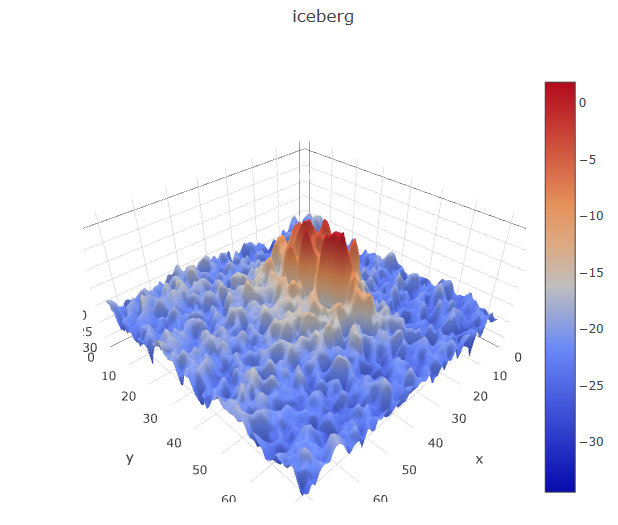
\includegraphics[width=\linewidth]{3diceberg}
\caption{iceberg image looks big}
\label{fig:3diceberg}
\end{figure}
\begin{figure}[ht]\centering
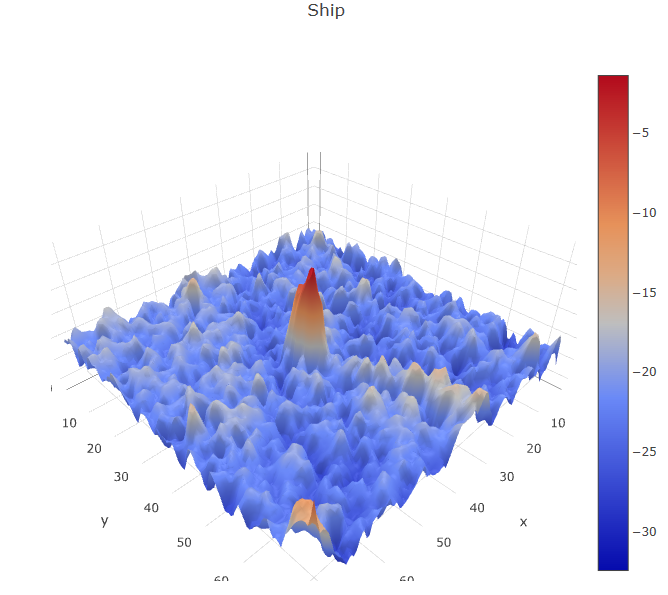
\includegraphics[width=\linewidth]{3dship}
\caption{ship image looks small as some needle}
\label{fig:3dship}
\end{figure}

From above 3-d iceberg and ship image, we can find that iceberg is bigger than ship,which arrives to the same conclusion as the first standard deviation and mean analysis.\\



\subsection{Methods}
We used Neural Network Models in Keras in our iceberg project.\

The focus of the Keras library is a model.The simplest model is defined in the Sequential class which is a linear stack of Layers.
we can create a Sequential model and define all of the layers in the constructor, we can add layers in the order of the computation we wish to perform.Layers of different type are a few properties in common, specifically their method of weight initialization and activation functions.There are a large number of core Layer types for standard neural networks.Some common and useful layer types you can choose from are Dense,dropout and Merge.
once the model is defined, next step is to compile it:using the compile() function and it accepts three important attributes, model optimizer, loss function and Metrics.
Then use fit() function to train model:Training both specifies the number of epochs to train on and the batch size.Epochs is the number of times that the model is exposed to the training dataset.Batch Size (batch\_size) is the number of training instances shown to the model before a weight update is performed.The fit function also allows for some basic evaluation of the model during training. You can set the validation\_split value to hold back a fraction of the training dataset for validation to be evaluated each epoch, or provide a validation\_data tuple of (X, y) of data to evaluate.Fitting the model returns a history object with details and metrics calculated for the model each epoch. This can be used for graphing model performance.
Once the model has been trained,we can use it to predict test data or new data.There are a number of different output types we can calculate from your trained model, each calculated using a different function call on our model object. For example
model.evaluate(),model.predict(),model.predict\_classes(), and model.predict\_proba(). In our iceberg project, we used model.predict\_proba() function.

\begin{figure}[ht]\centering
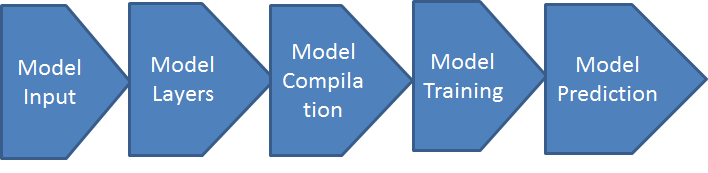
\includegraphics[width=\linewidth]{Kerasmodel}
\caption{Neural Network Models in Keras}
\label{fig:Kerasmodel}
\end{figure}

\begin{figure}[ht]\centering
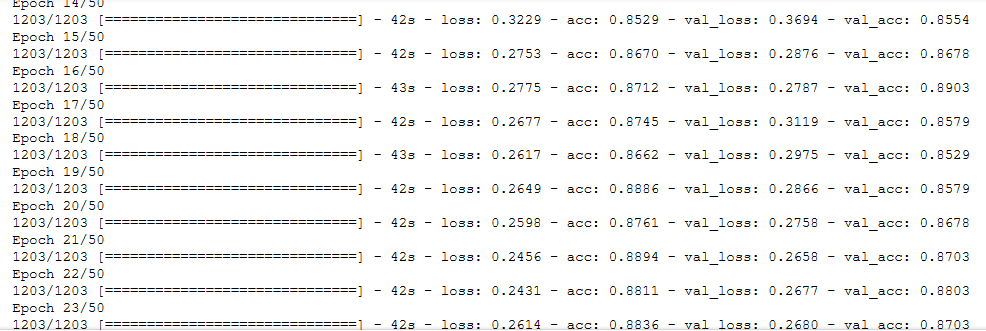
\includegraphics[width=\linewidth]{trainmodel}
\caption{Train model in keras}
\label{fig:trainmodel}
\end{figure}



%------------------------------------------------

\subsection{Results}
Our accuracy is about 87\%, which sounds good, but when it comes to the fact that the result can save lives, we believe we should be trying more.\\
We did try it for a variety of epochs, and we saw an increase in accuracy with more epochs we used.\\
\begin{figure}[H]\centering
	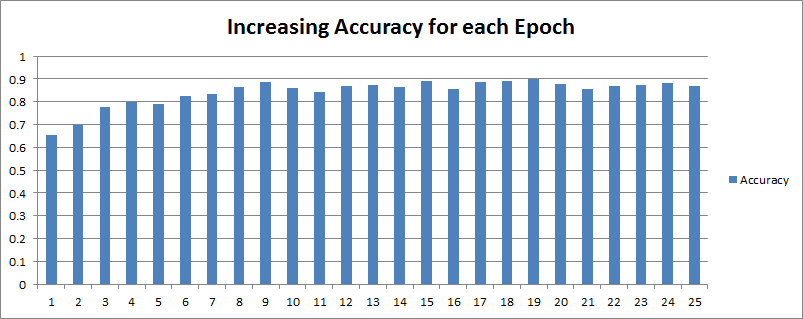
\includegraphics[width=\linewidth]{increasingaccuracy.png}
	\caption{accuracy increase with epoch}
	\label{fig:accuracy inc}
\end{figure}
As we can see we maxed at 19 epochs, which is shown below.\\
\begin{figure}[H]\centering
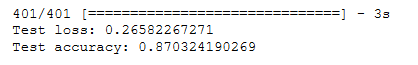
\includegraphics[width=\linewidth]{testaccuracy}
\caption{test accuracy}
\label{fig:testaccuracy}
\end{figure}
The validation was done using 5-Fold cross validation.\\
We randomly created test and train data from the cleaned training data, using 30\% for test and rest for train.
\subsection{Summary and Future Work}
The Iceberg Identification Challenge, was a really good one, we got to work on visual data. It is a very good challenge as the outcome of the challenge will be an implementation which would help identify icebergs and potentially save many lives.\\
We used a convolution neural networks model using Keras to create train and predict on the provided data. we got 87\% accuracy, which we believe is quite good.\\
With regards to future work.\\
\begin{enumerate}
	\item We would like to analyze our implementation to identify improvements.\\
	\item We would also like to implement algorithms like AdaBoost and check the accuracy.\\
\end{enumerate}
\section*{Acknowledgments} % The \section*{} command stops section numbering
First of all, we would take this opportunity to thank Prof. Dalkilic, who taught us a lot of important knowledge and skills in data mining, and at the same time provided us a lot of chance to do projects. Especially he encouraged us to participate the competition in Kaggle.\\ Secondly we would like to thank Marcin Malec (Prof. Dalkilic's AI), who answered a lot of questions from us and provided a lot of help.\\
\addcontentsline{toc}{section}{Acknowledgments} % Adds this section to the table of contents

\section*{Refrences}
\begin{enumerate}
	\item Keras Documentation. https://keras.io/getting-started/sequential-model-guide
	\item Perceptrons and Neural Networks. https://faroit.github.io/keras-docs/0.2.0/examples/
	\item Learning Deep networks in python. https://elitedatascience.com/keras-tutorial-deep-learning-in-python
	\item Multi-Layer Perceptron. https://machinelearningmastery.com/build-multi-layer-perceptron-neural-network-models-keras/
	\item Practical Approach to Naive Bayes. https://monkeylearn.com/blog/practical-explanation-naive-bayes-classifier/
\end{enumerate}
%----------------------------------------------------------------------------------------
%	REFERENCE LIST
%----------------------------------------------------------------------------------------

%----------------------------------------------------------------------------------------

\end{document}